\subsection{Robot}
\label{sub:robots}
Gli agenti che modellano il comportamento dei robot sono, di fatto, la componenete principale di tutto il sistema.
Sono i robot, e loro soltanto, a muoversi all'interno del territorio cercando i feriti e costruendo, nel mentre, la rete \textit{mesh}; nonostante abbiano un ruolo così fondamentale, questi agenti sono a tutti gli effetti dei \textit{reflexive agent with internal state}, il cui comportamento viene descritto di seguito.
È bene esplicitare, prima di proseguire, qual'è lo stato interno dell'agente descritto: in questo caso, lo stato interno è dato da un insieme di variabili; in particolare:
\begin{itemize}
	\item \texttt{target\_cell}, ovvero la cella di frontiera a cui il robot è diretto;
	\item \texttt{target\_path} è il cammino minimo che l'agente deve seguire per raggiungere la cella obiettivo dalla posizione attuale;
	\item \texttt{status} serve per indicare se il robot sta esplorando una cella, si sta muovendo, sta scegliendo la prossima cella obiettivo (o sta aspettando che nuove celle si aggiungano alla frontiera) oppure che si è rotto.
\end{itemize}
Per alleggerire la lettura del diagramma di flusso sottostante e per comodità di descrizione dell'agente la casistica del fallimento di un robot verrà descritta di seguito separatamente.
Inoltre, come già detto nella Sezione \ref{sec:environment}, questi agenti presentano un insieme di altre variabili che ne descrivono delle caratteristiche o che vengono sfruttate dall'agente per effettuare delle scelte a livello “microscopico” (\textit{e.g.}, quale cella scegliere come obiettivo); a queste si aggiungono tra ulteriori variaibli di interesse: la posizione in cui si trova l'agente, quella precedente e l'utilità della cella scelta come obiettivo prima che venisse modificata (variabile utilizzata per la gestione dei fallimenti dei robot).
Infine, a livello programmativo, sono presenti un insieme di variaibli atte a simulare il tempo che il robot trascorre per spostarsi da una posizione ad un'altra o per esplorare una cella. 

Durante la sua vita, l'agente valuta il suo stato interno e se sta mantenendo una connessione con la rete \textit{mesh} oppure no, in base a queste due condizioni prende delle decisioni “macroscopiche” su quali azioni effettuare (\textit{e.g.}, decide di rilasciare un ripetitore \textit{wi-fi} oppure continuare a muoversi verso l'obiettivo) come mostrato in Figura \ref{fig:robotworkflow}.
È importante far notare che il processo decisionale non avviene ad ogni \textit{step} della simulazione (cioè ad ogni secondo), ma solo quando lo stato interno del robot subisce delle modifiche.
\begin{figure}
	\centering
	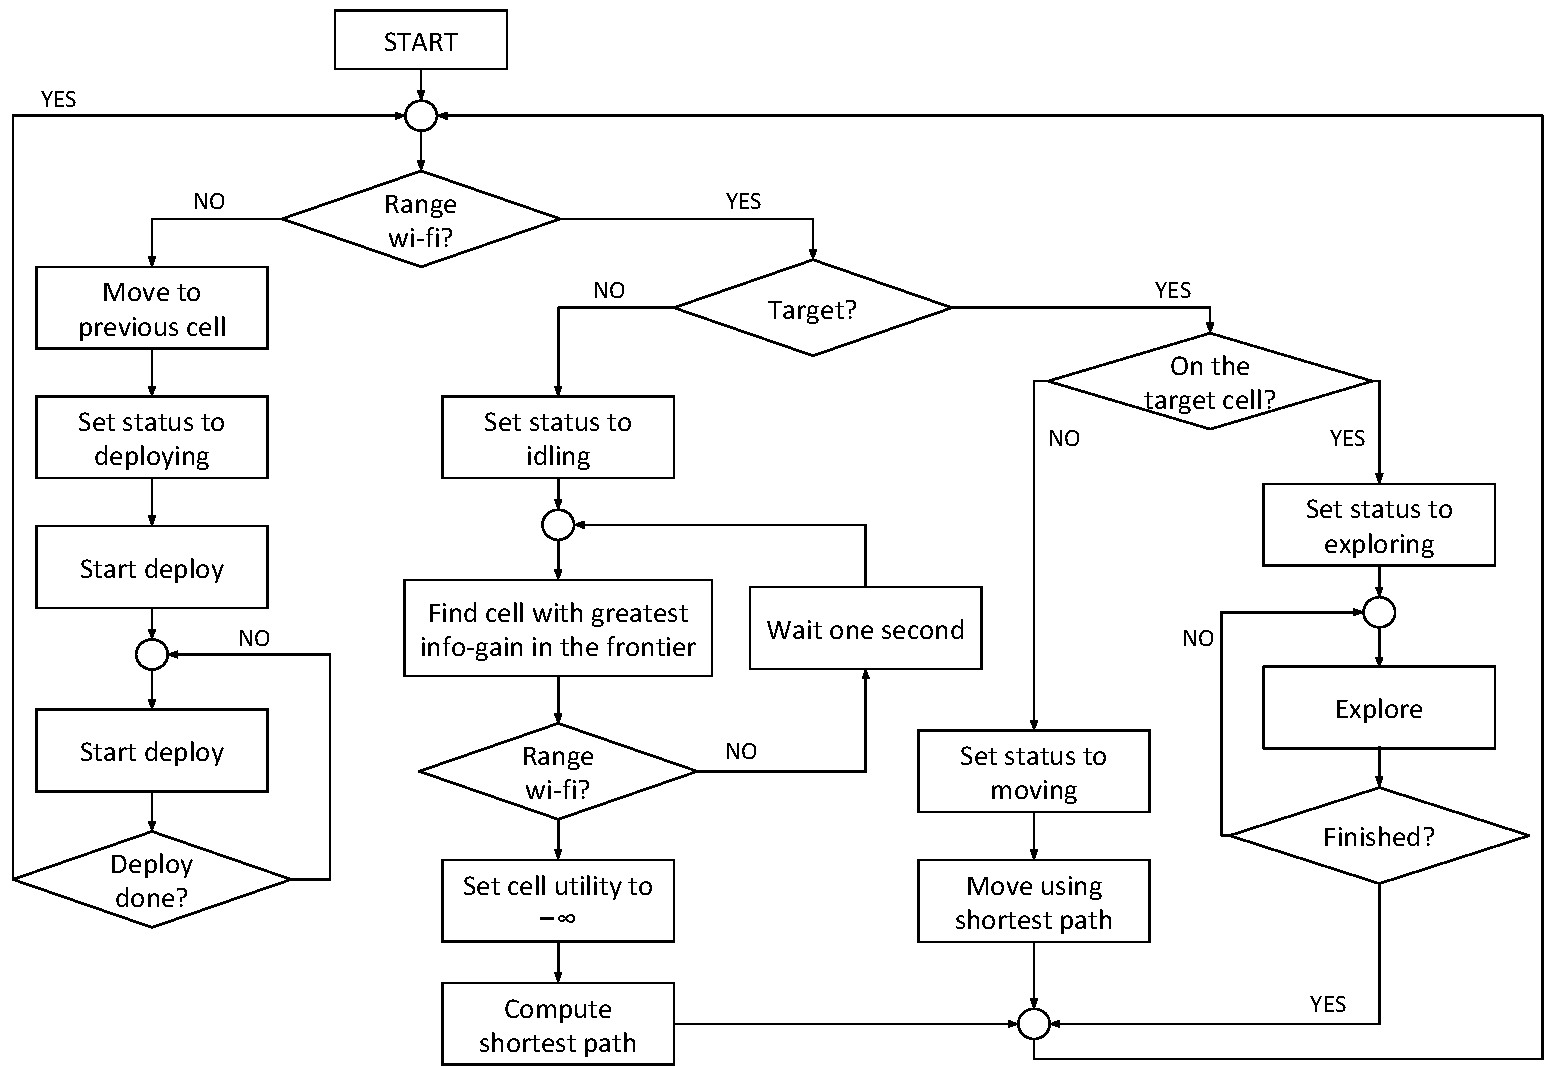
\includegraphics[width=1.0\linewidth]{images/Robot_workflow}
	\caption{Figura che rappresenta il processo decisionale che l'agente robot quando deve stabilire la sua prossima azione, tale processo si basa sullo stato interno del robot e sulla presenza (o assenza) di connessione con la rete \textit{mesh}; si noti, che quello appena descritto non avviene ad ogni step della simulazione ma solo quando lo stato interno dell'agente subisce dei cambiamenti.}
	\label{fig:robotworkflow}
\end{figure}
Per prima cosa, il robot valuta se è ancora all'interno della copertura \textit{wi-fi} poiché, per come è stato definito il metodo di comunicazione e coordinamento dei robot, risulta fondamentale che siano sempre in grado di comunicare tra loro.
Tale controllo risulta essere necessario farlo ogni volta che il robot, di fatto, si sposta di una cella perché è l'unico caso in cui si suppone che l'agente possa perdere la connessione uscendo dall'area coperta; per comodità e “pulizia” algoritmica viene anche effettuato nel caso in cuo il robot ha finito di esplorare una cella.
Quando il robot, muovendosi, esce dalla zona coperta, se ne accorge e allo \textit{step} successivo rientra immeditamente nella zona coperta iniziando il processo di rilascio del \textit{bean}: aggiorna il suo stato in fase di \textit{deploy}, iniziando poi il processo di rilascio il quale abbiamo supposto impieghi circa un 15 secondi (\textit{i.e.}, 15 \textit{step}) poiché il rilascio del ripetitore deve essere effettuato in un luogo e in modo sicuro.\\
Altrimenti, se il robot è in una zona coperta, la sua decisione viene determinata dal possedimento di una cella \textit{target}.
In particolare, se non possiede una cella obiettivo deve sceglierne una: per prima cosa, si mette in stato di \textit{idling}, ovvero lo stao rappresentante che il robot è fermo per calcolare il suo prossimo obiettivo oppure che non ha celle tra cui scegliere.
In seguito deve stabilire la cella “migliore” da esplorare; per far ciò, i robot sfruttano un concetto di \textit{information gain} (o \textit{info-gain}) \todo[inline]{qua mi sa che c'è da citare l'articolo dicendo cosa noi abbiamo cambiato rispetto a loro, puoi farlo te? Grazie DP} che è uno scalare che indica “quanta informazione può portare l'esplorazione di una cella”, ovvero più tale valore è alto più ad un agente conviene andare ad esplorare tale cella.
La Formula \ref{math:info-gain} è quella utilizzata dagli agenti per il calcolo dell'\textit{info-gain}, tale valore viene calcolato per ogni cella della frontiera.
\begin{equation}
	\label{math:info-gain}
	\textit{Information gain} = \rho+\mu-\alpha\omega
\end{equation}
In tale formula:
\begin{itemize}
	\item $\rho$ è la priorità della cella che risulta essere pari a zero tranne nei casi in cui la cella sia adiacente ad una cella in cui una vittima sia riuscita a segnalare la sua presenza;
	\item $\mu$ è l'utilità della cella;
	\item $\alpha$ è il parametro, già nominato in precedenza, che indica quanto il costo del percorso per raggiungere la cella d'interesse pesi nella scelta;
	\item $\omega$ è il costo, in termini di \textit{step} necessari per raggiungere la cella d'interesse.
\end{itemize}
Per il calcolo di $\omega$ per ogni cella della frontiera, viene computato il costo del cammino minimo sfruttando la rappresentazione interna del territorio che possegono (e condividono) i robot sotto forma di grafo; \textit{i.e.}, di fatto si calcolano insieme tutti i cammini minimi (e i loro costi) dalla cella in cui è presente il robot verso tutte le altre celle sfruttando l'algoritmo definito da Dijkstra.
Infine, verrà scelta la cella con \textit{info-gain} maggiore tra tutte le celle della frontiera, diventando così la cella \textit{target} dell'agente.
Se il robot è riuscito ad individuare la sua prossima cella obiettivo, imposta l'utilità di tale cella pari a $-\infty$ in modo che nessun altro agente scelga tale cella e poi \todo[inline]{perché la rimuoviamo in find best cell la cella dalal frotniera? non dovremmo rimuoverla quando il robot la esplora? per come abbiamo definito la frontiera quella cella è ancora in frotniera, come lo sistemiamo nella relazione? DP}.
Vi sono dei casi in cui è possibile che l'agente non riesca a stabilire il suo prossimo obiettivo perché non vi sono celle nella frontiera oppure perché tutte le celle hanno utilità pari a meno infinito e quindi stanno già venendo esplorate da un altro robot; in questi casi, i robot aspettano un secondo prima di riaggiornare la rappresentazione del territorio condivisa e poi cercano nuovamente una possibile cella.
% riduzione dell'utilità attorno alla cella scelta -> gamma
\todo[inline]{Anche questa riduzione non sarebbe da fare una volta che il robot arriva sulla cella e percepisce attorno? DP}
\todo[inline]]{Perché proprio diviso il radar radius? Puoi aggiungerlo te? Grazie DP}
% parametri
% metodo di comunicazione tra i robot
% metodologie di prioritizzazione
\todo[inline]{fallimenti parlarne altrove? DP}
\subsection{Ferito}
Questo agente rappresenta le persone ferite che sono disperse nell'area di interesse e necessitano di essere individuate e salvate, si noti che il loro salvataggio non fa parte di questo simulatore poiché le metodologie di salvataggio dipendono da troppi fattori che non possono venir considerati complessivamente in un simulatore (\textit{e.g.}, la loro possibilità di muoversi oppure se richiedono un intervento medico sul campo).
Il loro comportamento è stocastico ma basato su uno stato interno, di conseguenza tali agenti sono stati classificati come \textit{reflexive agent with internal state}, facendo riferimento alla classificazione proposta da Russell e Norvig \cite{russell2016}.
L'agente è molto semplice, possiede due attributi che lo descrivono: la posizione all'interno della griglia e lo stato interno; lo stato assume valore 0 nel momento in cui non è ancora stato trovato e 1 quando è stato trovato e quindi salvato successivamente.
Il suo comportamento, come detto, dipende dal suo stato interno, in particolare: 
\begin{itemize}
	\item finché tale agente non è stato individuato e la cella in cui si trova non è coperta dal \textit{wi-fi} non fa nulla;
	\item se si trova in una cella coperta e non è ancora stato individuato, ha una probabilità pari a $10^{-3}$ di segnalare la sua presenza collegandosi alla rete \textit{mesh}, tale probabilità risulta essere bassa perché bisogna considerare che ad ogni \textit{step} (un secondo di tempo d'orologio) della simulazione un ferito può segnalare la sua presenza ed inoltre non tutte le persone potrebbero aver accesso ad un telefono in una situazione critica;
	\item se è stato individuato da un robot o ha già segnalato la sua presenza, non fa altro che aspettare.
\end{itemize}
% Le due metodologie di prioritizzazione dei feriti le nasconderei sotto il cappuccio e ne parlerei nei robot DP